\documentclass[1p]{elsarticle_modified}
%\bibliographystyle{elsarticle-num}

%\usepackage[colorlinks]{hyperref}
%\usepackage{abbrmath_seonhwa} %\Abb, \Ascr, \Acal ,\Abf, \Afrak
\usepackage{amsfonts}
\usepackage{amssymb}
\usepackage{amsmath}
\usepackage{amsthm}
\usepackage{scalefnt}
\usepackage{amsbsy}
\usepackage{kotex}
\usepackage{caption}
\usepackage{subfig}
\usepackage{color}
\usepackage{graphicx}
\usepackage{xcolor} %% white, black, red, green, blue, cyan, magenta, yellow
\usepackage{float}
\usepackage{setspace}
\usepackage{hyperref}

\usepackage{tikz}
\usetikzlibrary{arrows}

\usepackage{multirow}
\usepackage{array} % fixed length table
\usepackage{hhline}

%%%%%%%%%%%%%%%%%%%%%
\makeatletter
\renewcommand*\env@matrix[1][\arraystretch]{%
	\edef\arraystretch{#1}%
	\hskip -\arraycolsep
	\let\@ifnextchar\new@ifnextchar
	\array{*\c@MaxMatrixCols c}}
\makeatother %https://tex.stackexchange.com/questions/14071/how-can-i-increase-the-line-spacing-in-a-matrix
%%%%%%%%%%%%%%%

\usepackage[normalem]{ulem}

\newcommand{\msout}[1]{\ifmmode\text{\sout{\ensuremath{#1}}}\else\sout{#1}\fi}
%SOURCE: \msout is \stkout macro in https://tex.stackexchange.com/questions/20609/strikeout-in-math-mode

\newcommand{\cancel}[1]{
	\ifmmode
	{\color{red}\msout{#1}}
	\else
	{\color{red}\sout{#1}}
	\fi
}

\newcommand{\add}[1]{
	{\color{blue}\uwave{#1}}
}

\newcommand{\replace}[2]{
	\ifmmode
	{\color{red}\msout{#1}}{\color{blue}\uwave{#2}}
	\else
	{\color{red}\sout{#1}}{\color{blue}\uwave{#2}}
	\fi
}

\newcommand{\Sol}{\mathcal{S}} %segment
\newcommand{\D}{D} %diagram
\newcommand{\A}{\mathcal{A}} %arc


%%%%%%%%%%%%%%%%%%%%%%%%%%%%%5 test

\def\sl{\operatorname{\textup{SL}}(2,\Cbb)}
\def\psl{\operatorname{\textup{PSL}}(2,\Cbb)}
\def\quan{\mkern 1mu \triangleright \mkern 1mu}

\theoremstyle{definition}
\newtheorem{thm}{Theorem}[section]
\newtheorem{prop}[thm]{Proposition}
\newtheorem{lem}[thm]{Lemma}
\newtheorem{ques}[thm]{Question}
\newtheorem{cor}[thm]{Corollary}
\newtheorem{defn}[thm]{Definition}
\newtheorem{exam}[thm]{Example}
\newtheorem{rmk}[thm]{Remark}
\newtheorem{alg}[thm]{Algorithm}

\newcommand{\I}{\sqrt{-1}}
\begin{document}

%\begin{frontmatter}
%
%\title{Boundary parabolic representations of knots up to 8 crossings}
%
%%% Group authors per affiliation:
%\author{Yunhi Cho} 
%\address{Department of Mathematics, University of Seoul, Seoul, Korea}
%\ead{yhcho@uos.ac.kr}
%
%
%\author{Seonhwa Kim} %\fnref{s_kim}}
%\address{Center for Geometry and Physics, Institute for Basic Science, Pohang, 37673, Korea}
%\ead{ryeona17@ibs.re.kr}
%
%\author{Hyuk Kim}
%\address{Department of Mathematical Sciences, Seoul National University, Seoul 08826, Korea}
%\ead{hyukkim@snu.ac.kr}
%
%\author{Seokbeom Yoon}
%\address{Department of Mathematical Sciences, Seoul National University, Seoul, 08826,  Korea}
%\ead{sbyoon15@snu.ac.kr}
%
%\begin{abstract}
%We find all boundary parabolic representation of knots up to 8 crossings.
%
%\end{abstract}
%\begin{keyword}
%    \MSC[2010] 57M25 
%\end{keyword}
%
%\end{frontmatter}

%\linenumbers
%\tableofcontents
%
\newcommand\colored[1]{\textcolor{white}{\rule[-0.35ex]{0.8em}{1.4ex}}\kern-0.8em\color{red} #1}%
%\newcommand\colored[1]{\textcolor{white}{ #1}\kern-2.17ex	\textcolor{white}{ #1}\kern-1.81ex	\textcolor{white}{ #1}\kern-2.15ex\color{red}#1	}

{\Large $\underline{12n_{0691}~(K12n_{0691})}$}

\setlength{\tabcolsep}{10pt}
\renewcommand{\arraystretch}{1.6}
\vspace{1cm}\begin{tabular}{m{100pt}>{\centering\arraybackslash}m{274pt}}
\multirow{5}{120pt}{
	\centering
	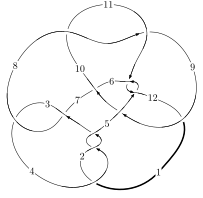
\includegraphics[width=112pt]{../../../GIT/diagram.site/Diagrams/png/2780_12n_0691.png}\\
\ \ \ A knot diagram\footnotemark}&
\allowdisplaybreaks
\textbf{Linearized knot diagam} \\
\cline{2-2}
 &
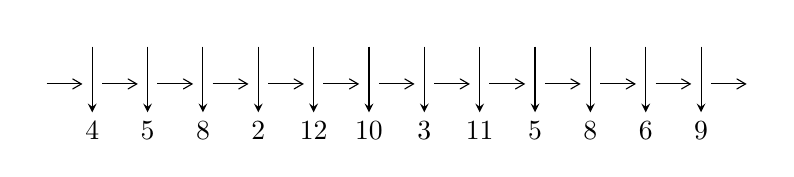
\begin{tikzpicture}[x=20pt, y=17pt]
	% nodes
	\node (C0) at (0, 0) {};
	\node (C1) at (1, 0) {};
	\node (C1U) at (1, +1) {};
	\node (C1D) at (1, -1) {4};

	\node (C2) at (2, 0) {};
	\node (C2U) at (2, +1) {};
	\node (C2D) at (2, -1) {5};

	\node (C3) at (3, 0) {};
	\node (C3U) at (3, +1) {};
	\node (C3D) at (3, -1) {8};

	\node (C4) at (4, 0) {};
	\node (C4U) at (4, +1) {};
	\node (C4D) at (4, -1) {2};

	\node (C5) at (5, 0) {};
	\node (C5U) at (5, +1) {};
	\node (C5D) at (5, -1) {12};

	\node (C6) at (6, 0) {};
	\node (C6U) at (6, +1) {};
	\node (C6D) at (6, -1) {10};

	\node (C7) at (7, 0) {};
	\node (C7U) at (7, +1) {};
	\node (C7D) at (7, -1) {3};

	\node (C8) at (8, 0) {};
	\node (C8U) at (8, +1) {};
	\node (C8D) at (8, -1) {11};

	\node (C9) at (9, 0) {};
	\node (C9U) at (9, +1) {};
	\node (C9D) at (9, -1) {5};

	\node (C10) at (10, 0) {};
	\node (C10U) at (10, +1) {};
	\node (C10D) at (10, -1) {8};

	\node (C11) at (11, 0) {};
	\node (C11U) at (11, +1) {};
	\node (C11D) at (11, -1) {6};

	\node (C12) at (12, 0) {};
	\node (C12U) at (12, +1) {};
	\node (C12D) at (12, -1) {9};
	\node (C13) at (13, 0) {};

	% arrows
	\draw[->,>={angle 60}]
	(C0) edge (C1) (C1) edge (C2) (C2) edge (C3) (C3) edge (C4) (C4) edge (C5) (C5) edge (C6) (C6) edge (C7) (C7) edge (C8) (C8) edge (C9) (C9) edge (C10) (C10) edge (C11) (C11) edge (C12) (C12) edge (C13) ;	\draw[->,>=stealth]
	(C1U) edge (C1D) (C2U) edge (C2D) (C3U) edge (C3D) (C4U) edge (C4D) (C5U) edge (C5D) (C6U) edge (C6D) (C7U) edge (C7D) (C8U) edge (C8D) (C9U) edge (C9D) (C10U) edge (C10D) (C11U) edge (C11D) (C12U) edge (C12D) ;
	\end{tikzpicture} \\
\hhline{~~} \\& 
\textbf{Solving Sequence} \\ \cline{2-2} 
 &
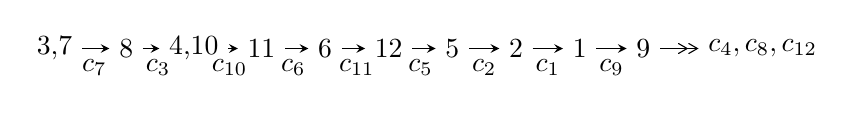
\begin{tikzpicture}[x=23pt, y=7pt]
	% node
	\node (A0) at (-1/8, 0) {3,7};
	\node (A1) at (1, 0) {8};
	\node (A2) at (33/16, 0) {4,10};
	\node (A3) at (25/8, 0) {11};
	\node (A4) at (33/8, 0) {6};
	\node (A5) at (41/8, 0) {12};
	\node (A6) at (49/8, 0) {5};
	\node (A7) at (57/8, 0) {2};
	\node (A8) at (65/8, 0) {1};
	\node (A9) at (73/8, 0) {9};
	\node (C1) at (1/2, -1) {$c_{7}$};
	\node (C2) at (3/2, -1) {$c_{3}$};
	\node (C3) at (21/8, -1) {$c_{10}$};
	\node (C4) at (29/8, -1) {$c_{6}$};
	\node (C5) at (37/8, -1) {$c_{11}$};
	\node (C6) at (45/8, -1) {$c_{5}$};
	\node (C7) at (53/8, -1) {$c_{2}$};
	\node (C8) at (61/8, -1) {$c_{1}$};
	\node (C9) at (69/8, -1) {$c_{9}$};
	\node (A10) at (11, 0) {$c_{4},c_{8},c_{12}$};

	% edge
	\draw[->,>=stealth]	
	(A0) edge (A1) (A1) edge (A2) (A2) edge (A3) (A3) edge (A4) (A4) edge (A5) (A5) edge (A6) (A6) edge (A7) (A7) edge (A8) (A8) edge (A9) ;
	\draw[->>,>={angle 60}]	
	(A9) edge (A10);
\end{tikzpicture} \\ 

\end{tabular} \\

\footnotetext{
The image of knot diagram is generated by the software ``\textbf{Draw programme}" developed by Andrew Bartholomew(\url{http://www.layer8.co.uk/maths/draw/index.htm\#Running-draw}), where we modified some parts for our purpose(\url{https://github.com/CATsTAILs/LinksPainter}).
}\phantom \\ \newline 
\centering \textbf{Ideals for irreducible components\footnotemark of $X_{\text{par}}$} 
 
\begin{align*}
I^u_{1}&=\langle 
16394625770 u^{16}+7361888468 u^{15}+\cdots+176471185595 b+67083506624,\\
\phantom{I^u_{1}}&\phantom{= \langle  }-638545424984 u^{16}+494483967338 u^{15}+\cdots+176471185595 a+990730965236,\\
\phantom{I^u_{1}}&\phantom{= \langle  }u^{17}- u^{16}+\cdots- u+1\rangle \\
I^u_{2}&=\langle 
u^7-2 u^5+3 u^3+b-2 u-1,\;-2 u^7-2 u^6+3 u^5+4 u^4-4 u^3-4 u^2+a+3 u+4,\\
\phantom{I^u_{2}}&\phantom{= \langle  }u^8+u^7- u^6-2 u^5+u^4+2 u^3-2 u-1\rangle \\
I^u_{3}&=\langle 
2.09794\times10^{14} u^{15}-1.54864\times10^{15} u^{14}+\cdots+1.00649\times10^{18} b-1.27599\times10^{18},\\
\phantom{I^u_{3}}&\phantom{= \langle  }3.01917\times10^{14} u^{15}-2.04767\times10^{15} u^{14}+\cdots+2.01298\times10^{18} a-2.50594\times10^{18},\\
\phantom{I^u_{3}}&\phantom{= \langle  }u^{16}- u^{15}+\cdots+640 u+256\rangle \\
\\
I^v_{1}&=\langle 
a,\;669 v^7+1791 v^6+1344 v^5-4076 v^4-11099 v^3+10779 v^2+887 b+981 v-54,\\
\phantom{I^v_{1}}&\phantom{= \langle  }v^8+2 v^7-8 v^5-13 v^4+28 v^3-7 v^2-3 v+1\rangle \\
\end{align*}
\raggedright * 4 irreducible components of $\dim_{\mathbb{C}}=0$, with total 49 representations.\\
\footnotetext{All coefficients of polynomials are rational numbers. But the coefficients are sometimes approximated in decimal forms when there is not enough margin.}
\newpage
\renewcommand{\arraystretch}{1}
\centering \section*{I. $I^u_{1}= \langle 1.64\times10^{10} u^{16}+7.36\times10^{9} u^{15}+\cdots+1.76\times10^{11} b+6.71\times10^{10},\;-6.39\times10^{11} u^{16}+4.94\times10^{11} u^{15}+\cdots+1.76\times10^{11} a+9.91\times10^{11},\;u^{17}- u^{16}+\cdots- u+1 \rangle$}
\flushleft \textbf{(i) Arc colorings}\\
\begin{tabular}{m{7pt} m{180pt} m{7pt} m{180pt} }
\flushright $a_{3}=$&$\begin{pmatrix}0\\u\end{pmatrix}$ \\
\flushright $a_{7}=$&$\begin{pmatrix}1\\0\end{pmatrix}$ \\
\flushright $a_{8}=$&$\begin{pmatrix}1\\u^2\end{pmatrix}$ \\
\flushright $a_{4}=$&$\begin{pmatrix}- u\\- u^3+u\end{pmatrix}$ \\
\flushright $a_{10}=$&$\begin{pmatrix}3.61841 u^{16}-2.80207 u^{15}+\cdots-2.45782 u-5.61412\\-0.0929026 u^{16}-0.0417172 u^{15}+\cdots-1.35646 u-0.380139\end{pmatrix}$ \\
\flushright $a_{11}=$&$\begin{pmatrix}3.73975 u^{16}-3.05444 u^{15}+\cdots-3.90343 u-6.05033\\0.0499193 u^{16}-0.188766 u^{15}+\cdots-1.60883 u-0.249100\end{pmatrix}$ \\
\flushright $a_{6}=$&$\begin{pmatrix}3.51660 u^{16}-1.48871 u^{15}+\cdots+10.1705 u-1.96079\\-0.183505 u^{16}-0.0479152 u^{15}+\cdots-0.736610 u-1.19077\end{pmatrix}$ \\
\flushright $a_{12}=$&$\begin{pmatrix}4.59450 u^{16}-5.53078 u^{15}+\cdots-7.72513 u-11.9429\\-0.302029 u^{16}-0.353052 u^{15}+\cdots-4.64374 u+0.978839\end{pmatrix}$ \\
\flushright $a_{5}=$&$\begin{pmatrix}0.436207 u^{16}-0.314873 u^{15}+\cdots-2.65787 u-1.88181\\-0.318145 u^{16}+0.389552 u^{15}+\cdots+0.690292 u-0.0974507\end{pmatrix}$ \\
\flushright $a_{2}=$&$\begin{pmatrix}-0.249100 u^{16}+0.199181 u^{15}+\cdots+1.65271 u+1.85793\\-0.0482596 u^{16}-0.0849909 u^{15}+\cdots+1.20435 u+0.0738023\end{pmatrix}$ \\
\flushright $a_{1}=$&$\begin{pmatrix}-0.118062 u^{16}-0.0746790 u^{15}+\cdots+1.96758 u+1.97926\\-0.175071 u^{16}+0.0850715 u^{15}+\cdots+0.615613 u+0.0952905\end{pmatrix}$ \\
\flushright $a_{9}=$&$\begin{pmatrix}3.49708 u^{16}-2.54969 u^{15}+\cdots-1.01221 u-5.17792\\-0.164310 u^{16}+0.0417260 u^{15}+\cdots-0.940864 u-0.698283\end{pmatrix}$\\&\end{tabular}
\flushleft \textbf{(ii) Obstruction class $= -1$}\\~\\
\flushleft \textbf{(iii) Cusp Shapes $= \frac{2048919230872}{176471185595} u^{16}-\frac{1391303845096}{176471185595} u^{15}+\cdots-\frac{3163149744064}{176471185595} u-\frac{6932356318654}{176471185595}$}\\~\\
\newpage\renewcommand{\arraystretch}{1}
\flushleft \textbf{(iv) u-Polynomials at the component}\newline \\
\begin{tabular}{m{50pt}|m{274pt}}
Crossings & \hspace{64pt}u-Polynomials at each crossing \\
\hline $$\begin{aligned}c_{1},c_{2},c_{4}\\c_{8},c_{10}\end{aligned}$$&$\begin{aligned}
&u^{17}-7 u^{16}+\cdots-5 u-1
\end{aligned}$\\
\hline $$\begin{aligned}c_{3},c_{7},c_{9}\end{aligned}$$&$\begin{aligned}
&u^{17}- u^{16}+\cdots- u+1
\end{aligned}$\\
\hline $$\begin{aligned}c_{5},c_{11}\end{aligned}$$&$\begin{aligned}
&u^{17}- u^{16}+\cdots+3 u-1
\end{aligned}$\\
\hline $$\begin{aligned}c_{6}\end{aligned}$$&$\begin{aligned}
&u^{17}+u^{16}+\cdots-699 u+199
\end{aligned}$\\
\hline $$\begin{aligned}c_{12}\end{aligned}$$&$\begin{aligned}
&u^{17}+3 u^{16}+\cdots-263 u-83
\end{aligned}$\\
\hline
\end{tabular}\\~\\
\newpage\renewcommand{\arraystretch}{1}
\flushleft \textbf{(v) Riley Polynomials at the component}\newline \\
\begin{tabular}{m{50pt}|m{274pt}}
Crossings & \hspace{64pt}Riley Polynomials at each crossing \\
\hline $$\begin{aligned}c_{1},c_{2},c_{4}\\c_{8},c_{10}\end{aligned}$$&$\begin{aligned}
&y^{17}-13 y^{16}+\cdots+21 y-1
\end{aligned}$\\
\hline $$\begin{aligned}c_{3},c_{7},c_{9}\end{aligned}$$&$\begin{aligned}
&y^{17}+15 y^{16}+\cdots+13 y-1
\end{aligned}$\\
\hline $$\begin{aligned}c_{5},c_{11}\end{aligned}$$&$\begin{aligned}
&y^{17}+11 y^{16}+\cdots+25 y-1
\end{aligned}$\\
\hline $$\begin{aligned}c_{6}\end{aligned}$$&$\begin{aligned}
&y^{17}+27 y^{16}+\cdots+947097 y-39601
\end{aligned}$\\
\hline $$\begin{aligned}c_{12}\end{aligned}$$&$\begin{aligned}
&y^{17}+7 y^{16}+\cdots+91413 y-6889
\end{aligned}$\\
\hline
\end{tabular}\\~\\
\newpage\flushleft \textbf{(vi) Complex Volumes and Cusp Shapes}
$$\begin{array}{c|c|c}  
\text{Solutions to }I^u_{1}& \I (\text{vol} + \sqrt{-1}CS) & \text{Cusp shape}\\
 \hline 
\begin{aligned}
u &= -0.764077 + 0.442209 I \\
a &= \phantom{-}0.346619 + 0.162821 I \\
b &= -0.958812 + 0.033588 I\end{aligned}
 & -4.55533 + 6.93072 I & -21.1582 - 11.9778 I \\ \hline\begin{aligned}
u &= -0.764077 - 0.442209 I \\
a &= \phantom{-}0.346619 - 0.162821 I \\
b &= -0.958812 - 0.033588 I\end{aligned}
 & -4.55533 - 6.93072 I & -21.1582 + 11.9778 I \\ \hline\begin{aligned}
u &= \phantom{-}0.791671\phantom{ +0.000000I} \\
a &= \phantom{-}0.322502\phantom{ +0.000000I} \\
b &= -1.02671\phantom{ +0.000000I}\end{aligned}
 & -8.70952\phantom{ +0.000000I} & -30.7710\phantom{ +0.000000I} \\ \hline\begin{aligned}
u &= -0.753921 + 0.115715 I \\
a &= \phantom{-}1.18926 - 1.58502 I \\
b &= \phantom{-}1.125680 - 0.771688 I\end{aligned}
 & -0.77832 - 2.01331 I & -15.1488 + 1.3786 I \\ \hline\begin{aligned}
u &= -0.753921 - 0.115715 I \\
a &= \phantom{-}1.18926 + 1.58502 I \\
b &= \phantom{-}1.125680 + 0.771688 I\end{aligned}
 & -0.77832 + 2.01331 I & -15.1488 - 1.3786 I \\ \hline\begin{aligned}
u &= \phantom{-}0.502094 + 0.490826 I \\
a &= \phantom{-}1.152440 + 0.058194 I \\
b &= -0.008463 + 0.987921 I\end{aligned}
 & \phantom{-}2.49540 - 2.02523 I & -6.20824 + 3.33819 I \\ \hline\begin{aligned}
u &= \phantom{-}0.502094 - 0.490826 I \\
a &= \phantom{-}1.152440 - 0.058194 I \\
b &= -0.008463 - 0.987921 I\end{aligned}
 & \phantom{-}2.49540 + 2.02523 I & -6.20824 - 3.33819 I \\ \hline\begin{aligned}
u &= \phantom{-}0.291694 + 0.477697 I \\
a &= \phantom{-}7.34853 + 5.73057 I \\
b &= -1.56713 + 1.11619 I\end{aligned}
 & -2.45442 + 0.76114 I & -1.7282 + 15.9915 I \\ \hline\begin{aligned}
u &= \phantom{-}0.291694 - 0.477697 I \\
a &= \phantom{-}7.34853 - 5.73057 I \\
b &= -1.56713 - 1.11619 I\end{aligned}
 & -2.45442 - 0.76114 I & -1.7282 - 15.9915 I \\ \hline\begin{aligned}
u &= -0.439135\phantom{ +0.000000I} \\
a &= \phantom{-}0.949461\phantom{ +0.000000I} \\
b &= \phantom{-}0.384048\phantom{ +0.000000I}\end{aligned}
 & -0.644803\phantom{ +0.000000I} & -15.2830\phantom{ +0.000000I}\\
 \hline 
 \end{array}$$\newpage$$\begin{array}{c|c|c}  
\text{Solutions to }I^u_{1}& \I (\text{vol} + \sqrt{-1}CS) & \text{Cusp shape}\\
 \hline 
\begin{aligned}
u &= \phantom{-}0.432752\phantom{ +0.000000I} \\
a &= -6.06938\phantom{ +0.000000I} \\
b &= -0.248275\phantom{ +0.000000I}\end{aligned}
 & -2.91990\phantom{ +0.000000I} & -47.5300\phantom{ +0.000000I} \\ \hline\begin{aligned}
u &= \phantom{-}0.78485 + 1.87131 I \\
a &= \phantom{-}0.345543 - 0.823882 I \\
b &= \phantom{-}0.13775 + 2.40985 I\end{aligned}
 & \phantom{-}11.20130 - 3.50827 I & -11.32341 + 1.79574 I \\ \hline\begin{aligned}
u &= \phantom{-}0.78485 - 1.87131 I \\
a &= \phantom{-}0.345543 + 0.823882 I \\
b &= \phantom{-}0.13775 - 2.40985 I\end{aligned}
 & \phantom{-}11.20130 + 3.50827 I & -11.32341 - 1.79574 I \\ \hline\begin{aligned}
u &= -0.93651 + 1.91501 I \\
a &= \phantom{-}0.272274 + 0.835217 I \\
b &= \phantom{-}0.86840 - 2.32205 I\end{aligned}
 & \phantom{-}6.80306 + 8.74093 I & -14.7558 - 4.0661 I \\ \hline\begin{aligned}
u &= -0.93651 - 1.91501 I \\
a &= \phantom{-}0.272274 - 0.835217 I \\
b &= \phantom{-}0.86840 + 2.32205 I\end{aligned}
 & \phantom{-}6.80306 - 8.74093 I & -14.7558 + 4.0661 I \\ \hline\begin{aligned}
u &= \phantom{-}0.98322 + 2.02620 I \\
a &= \phantom{-}0.244045 - 0.883210 I \\
b &= \phantom{-}1.34803 + 2.71046 I\end{aligned}
 & \phantom{-}10.6972 - 14.1953 I & -12.00000 + 6.60789 I \\ \hline\begin{aligned}
u &= \phantom{-}0.98322 - 2.02620 I \\
a &= \phantom{-}0.244045 + 0.883210 I \\
b &= \phantom{-}1.34803 - 2.71046 I\end{aligned}
 & \phantom{-}10.6972 + 14.1953 I & -12.00000 - 6.60789 I\\
 \hline 
 \end{array}$$\newpage\newpage\renewcommand{\arraystretch}{1}
\centering \section*{II. $I^u_{2}= \langle u^7-2 u^5+3 u^3+b-2 u-1,\;-2 u^7-2 u^6+\cdots+a+4,\;u^8+u^7- u^6-2 u^5+u^4+2 u^3-2 u-1 \rangle$}
\flushleft \textbf{(i) Arc colorings}\\
\begin{tabular}{m{7pt} m{180pt} m{7pt} m{180pt} }
\flushright $a_{3}=$&$\begin{pmatrix}0\\u\end{pmatrix}$ \\
\flushright $a_{7}=$&$\begin{pmatrix}1\\0\end{pmatrix}$ \\
\flushright $a_{8}=$&$\begin{pmatrix}1\\u^2\end{pmatrix}$ \\
\flushright $a_{4}=$&$\begin{pmatrix}- u\\- u^3+u\end{pmatrix}$ \\
\flushright $a_{10}=$&$\begin{pmatrix}2 u^7+2 u^6-3 u^5-4 u^4+4 u^3+4 u^2-3 u-4\\- u^7+2 u^5-3 u^3+2 u+1\end{pmatrix}$ \\
\flushright $a_{11}=$&$\begin{pmatrix}2 u^7+2 u^6-3 u^5-4 u^4+4 u^3+4 u^2-3 u-5\\- u^7+2 u^5-3 u^3- u^2+2 u+1\end{pmatrix}$ \\
\flushright $a_{6}=$&$\begin{pmatrix}2 u^7+2 u^6-4 u^5-4 u^4+5 u^3+4 u^2-4 u-1\\- u^7+u^5- u^3+2 u^2-1\end{pmatrix}$ \\
\flushright $a_{12}=$&$\begin{pmatrix}2 u^6-4 u^4+7 u^2- u-5\\-2 u^7- u^6+4 u^5+3 u^4-5 u^3-4 u^2+3 u+2\end{pmatrix}$ \\
\flushright $a_{5}=$&$\begin{pmatrix}u^4- u^2+1\\- u^4\end{pmatrix}$ \\
\flushright $a_{2}=$&$\begin{pmatrix}u^6- u^4+2 u^2-1\\- u^7- u^6+2 u^5+u^4-2 u^3-2 u^2+2 u+1\end{pmatrix}$ \\
\flushright $a_{1}=$&$\begin{pmatrix}u^2-1\\- u^2\end{pmatrix}$ \\
\flushright $a_{9}=$&$\begin{pmatrix}2 u^7+2 u^6-3 u^5-4 u^4+4 u^3+4 u^2-3 u-4\\- u^7+2 u^5-3 u^3+2 u+1\end{pmatrix}$\\&\end{tabular}
\flushleft \textbf{(ii) Obstruction class $= 1$}\\~\\
\flushleft \textbf{(iii) Cusp Shapes $= - u^7-4 u^6+2 u^5+5 u^4-3 u^3-5 u^2+5 u-10$}\\~\\
\newpage\renewcommand{\arraystretch}{1}
\flushleft \textbf{(iv) u-Polynomials at the component}\newline \\
\begin{tabular}{m{50pt}|m{274pt}}
Crossings & \hspace{64pt}u-Polynomials at each crossing \\
\hline $$\begin{aligned}c_{1},c_{2}\end{aligned}$$&$\begin{aligned}
&u^8+u^7-3 u^6-2 u^5+3 u^4+2 u-1
\end{aligned}$\\
\hline $$\begin{aligned}c_{3}\end{aligned}$$&$\begin{aligned}
&u^8- u^7- u^6+2 u^5+u^4-2 u^3+2 u-1
\end{aligned}$\\
\hline $$\begin{aligned}c_{4}\end{aligned}$$&$\begin{aligned}
&u^8- u^7-3 u^6+2 u^5+3 u^4-2 u-1
\end{aligned}$\\
\hline $$\begin{aligned}c_{5}\end{aligned}$$&$\begin{aligned}
&u^8+3 u^7+7 u^6+10 u^5+11 u^4+10 u^3+6 u^2+4 u+1
\end{aligned}$\\
\hline $$\begin{aligned}c_{6}\end{aligned}$$&$\begin{aligned}
&u^8-2 u^7- u^6+5 u^5+4 u^4-17 u^3+17 u^2-7 u+1
\end{aligned}$\\
\hline $$\begin{aligned}c_{7}\end{aligned}$$&$\begin{aligned}
&u^8+u^7- u^6-2 u^5+u^4+2 u^3-2 u-1
\end{aligned}$\\
\hline $$\begin{aligned}c_{8}\end{aligned}$$&$\begin{aligned}
&(u-1)^8
\end{aligned}$\\
\hline $$\begin{aligned}c_{9}\end{aligned}$$&$\begin{aligned}
&u^8
\end{aligned}$\\
\hline $$\begin{aligned}c_{10}\end{aligned}$$&$\begin{aligned}
&(u+1)^8
\end{aligned}$\\
\hline $$\begin{aligned}c_{11}\end{aligned}$$&$\begin{aligned}
&u^8-3 u^7+7 u^6-10 u^5+11 u^4-10 u^3+6 u^2-4 u+1
\end{aligned}$\\
\hline $$\begin{aligned}c_{12}\end{aligned}$$&$\begin{aligned}
&u^8+3 u^7+6 u^6+7 u^5+13 u^4+11 u^3+4 u^2+3 u+1
\end{aligned}$\\
\hline
\end{tabular}\\~\\
\newpage\renewcommand{\arraystretch}{1}
\flushleft \textbf{(v) Riley Polynomials at the component}\newline \\
\begin{tabular}{m{50pt}|m{274pt}}
Crossings & \hspace{64pt}Riley Polynomials at each crossing \\
\hline $$\begin{aligned}c_{1},c_{2},c_{4}\end{aligned}$$&$\begin{aligned}
&y^8-7 y^7+19 y^6-22 y^5+3 y^4+14 y^3-6 y^2-4 y+1
\end{aligned}$\\
\hline $$\begin{aligned}c_{3},c_{7}\end{aligned}$$&$\begin{aligned}
&y^8-3 y^7+7 y^6-10 y^5+11 y^4-10 y^3+6 y^2-4 y+1
\end{aligned}$\\
\hline $$\begin{aligned}c_{5},c_{11}\end{aligned}$$&$\begin{aligned}
&y^8+5 y^7+11 y^6+6 y^5-17 y^4-34 y^3-22 y^2-4 y+1
\end{aligned}$\\
\hline $$\begin{aligned}c_{6}\end{aligned}$$&$\begin{aligned}
&y^8-6 y^7+29 y^6-67 y^5+126 y^4-85 y^3+59 y^2-15 y+1
\end{aligned}$\\
\hline $$\begin{aligned}c_{8},c_{10}\end{aligned}$$&$\begin{aligned}
&(y-1)^8
\end{aligned}$\\
\hline $$\begin{aligned}c_{9}\end{aligned}$$&$\begin{aligned}
&y^8
\end{aligned}$\\
\hline $$\begin{aligned}c_{12}\end{aligned}$$&$\begin{aligned}
&y^8+3 y^7+20 y^6+49 y^5+47 y^4-47 y^3-24 y^2- y+1
\end{aligned}$\\
\hline
\end{tabular}\\~\\
\newpage\flushleft \textbf{(vi) Complex Volumes and Cusp Shapes}
$$\begin{array}{c|c|c}  
\text{Solutions to }I^u_{2}& \I (\text{vol} + \sqrt{-1}CS) & \text{Cusp shape}\\
 \hline 
\begin{aligned}
u &= -0.570868 + 0.730671 I \\
a &= \phantom{-}1.72219 - 2.56817 I \\
b &= -1.50065 - 0.90255 I\end{aligned}
 & -2.68559 - 1.13123 I & -18.1377 + 5.3065 I \\ \hline\begin{aligned}
u &= -0.570868 - 0.730671 I \\
a &= \phantom{-}1.72219 + 2.56817 I \\
b &= -1.50065 + 0.90255 I\end{aligned}
 & -2.68559 + 1.13123 I & -18.1377 - 5.3065 I \\ \hline\begin{aligned}
u &= \phantom{-}0.855237 + 0.665892 I \\
a &= -0.658590 - 0.551963 I \\
b &= \phantom{-}1.43900 - 0.90910 I\end{aligned}
 & \phantom{-}0.51448 - 2.57849 I & -10.11893 + 3.45077 I \\ \hline\begin{aligned}
u &= \phantom{-}0.855237 - 0.665892 I \\
a &= -0.658590 + 0.551963 I \\
b &= \phantom{-}1.43900 + 0.90910 I\end{aligned}
 & \phantom{-}0.51448 + 2.57849 I & -10.11893 - 3.45077 I \\ \hline\begin{aligned}
u &= \phantom{-}1.09818\phantom{ +0.000000I} \\
a &= -0.421763\phantom{ +0.000000I} \\
b &= \phantom{-}0.491355\phantom{ +0.000000I}\end{aligned}
 & -8.14766\phantom{ +0.000000I} & -12.9880\phantom{ +0.000000I} \\ \hline\begin{aligned}
u &= -1.031810 + 0.655470 I \\
a &= -0.420504 - 0.057447 I \\
b &= \phantom{-}0.655281 + 0.532312 I\end{aligned}
 & -4.02461 + 6.44354 I & -10.82984 - 2.68172 I \\ \hline\begin{aligned}
u &= -1.031810 - 0.655470 I \\
a &= -0.420504 + 0.057447 I \\
b &= \phantom{-}0.655281 - 0.532312 I\end{aligned}
 & -4.02461 - 6.44354 I & -10.82984 + 2.68172 I \\ \hline\begin{aligned}
u &= -0.603304\phantom{ +0.000000I} \\
a &= -1.86442\phantom{ +0.000000I} \\
b &= \phantom{-}0.321397\phantom{ +0.000000I}\end{aligned}
 & -2.48997\phantom{ +0.000000I} & -13.8390\phantom{ +0.000000I}\\
 \hline 
 \end{array}$$\newpage\newpage\renewcommand{\arraystretch}{1}
\centering \section*{III. $I^u_{3}= \langle 2.10\times10^{14} u^{15}-1.55\times10^{15} u^{14}+\cdots+1.01\times10^{18} b-1.28\times10^{18},\;3.02\times10^{14} u^{15}-2.05\times10^{15} u^{14}+\cdots+2.01\times10^{18} a-2.51\times10^{18},\;u^{16}- u^{15}+\cdots+640 u+256 \rangle$}
\flushleft \textbf{(i) Arc colorings}\\
\begin{tabular}{m{7pt} m{180pt} m{7pt} m{180pt} }
\flushright $a_{3}=$&$\begin{pmatrix}0\\u\end{pmatrix}$ \\
\flushright $a_{7}=$&$\begin{pmatrix}1\\0\end{pmatrix}$ \\
\flushright $a_{8}=$&$\begin{pmatrix}1\\u^2\end{pmatrix}$ \\
\flushright $a_{4}=$&$\begin{pmatrix}- u\\- u^3+u\end{pmatrix}$ \\
\flushright $a_{10}=$&$\begin{pmatrix}-0.000149985 u^{15}+0.00101723 u^{14}+\cdots+0.522231 u+1.24489\\-0.000208441 u^{15}+0.00153866 u^{14}+\cdots+0.527819 u+1.26776\end{pmatrix}$ \\
\flushright $a_{11}=$&$\begin{pmatrix}0.000149985 u^{15}-0.00101723 u^{14}+\cdots-0.522231 u-0.244888\\-0.000391498 u^{15}+0.00253027 u^{14}+\cdots+1.56110 u+1.71179\end{pmatrix}$ \\
\flushright $a_{6}=$&$\begin{pmatrix}0.0000210778 u^{15}-0.00137312 u^{14}+\cdots-1.23583 u-0.524902\\0.000823010 u^{15}-0.00190398 u^{14}+\cdots-1.08393 u-1.43592\end{pmatrix}$ \\
\flushright $a_{12}=$&$\begin{pmatrix}-0.000987334 u^{15}+0.000332252 u^{14}+\cdots-1.64360 u-0.285638\\-0.00263050 u^{15}+0.00407270 u^{14}+\cdots-2.52850 u+0.754844\end{pmatrix}$ \\
\flushright $a_{5}=$&$\begin{pmatrix}-0.000548337 u^{15}-0.000148181 u^{14}+\cdots-1.41913 u-0.208839\\0.00209134 u^{15}-0.00192142 u^{14}+\cdots+1.92702 u+0.216705\end{pmatrix}$ \\
\flushright $a_{2}=$&$\begin{pmatrix}-0.000318911 u^{15}+0.000923900 u^{14}+\cdots+0.0782544 u+0.170443\\0.0000474371 u^{15}+0.00190210 u^{14}+\cdots+1.03533 u-0.116481\end{pmatrix}$ \\
\flushright $a_{1}=$&$\begin{pmatrix}-0.00154300 u^{15}+0.00206961 u^{14}+\cdots-0.507891 u-0.00786525\\0.00175647 u^{15}+0.00275194 u^{14}+\cdots+1.98501 u+0.0818943\end{pmatrix}$ \\
\flushright $a_{9}=$&$\begin{pmatrix}-0.000675440 u^{15}+0.000547485 u^{14}+\cdots-1.09374 u+0.615472\\0.00211859 u^{15}-0.000320222 u^{14}+\cdots+3.48674 u+2.29159\end{pmatrix}$\\&\end{tabular}
\flushleft \textbf{(ii) Obstruction class $= -1$}\\~\\
\flushleft \textbf{(iii) Cusp Shapes $= \frac{4129940980039711}{1006491371550221696} u^{15}-\frac{3800282985571637}{1006491371550221696} u^{14}+\cdots+\frac{45304359399533900}{7863213840236107} u-\frac{73541352487366340}{7863213840236107}$}\\~\\
\newpage\renewcommand{\arraystretch}{1}
\flushleft \textbf{(iv) u-Polynomials at the component}\newline \\
\begin{tabular}{m{50pt}|m{274pt}}
Crossings & \hspace{64pt}u-Polynomials at each crossing \\
\hline $$\begin{aligned}c_{1},c_{2},c_{4}\\c_{8},c_{10}\end{aligned}$$&$\begin{aligned}
&u^{16}-3 u^{15}+\cdots-8 u+1
\end{aligned}$\\
\hline $$\begin{aligned}c_{3},c_{7},c_{9}\end{aligned}$$&$\begin{aligned}
&u^{16}- u^{15}+\cdots+640 u+256
\end{aligned}$\\
\hline $$\begin{aligned}c_{5},c_{11}\end{aligned}$$&$\begin{aligned}
&(u^8- u^7+3 u^6-2 u^5+3 u^4-2 u^3-1)^2
\end{aligned}$\\
\hline $$\begin{aligned}c_{6}\end{aligned}$$&$\begin{aligned}
&u^{16}+3 u^{15}+\cdots+2169 u+361
\end{aligned}$\\
\hline $$\begin{aligned}c_{12}\end{aligned}$$&$\begin{aligned}
&u^{16}-4 u^{15}+\cdots-189 u+297
\end{aligned}$\\
\hline
\end{tabular}\\~\\
\newpage\renewcommand{\arraystretch}{1}
\flushleft \textbf{(v) Riley Polynomials at the component}\newline \\
\begin{tabular}{m{50pt}|m{274pt}}
Crossings & \hspace{64pt}Riley Polynomials at each crossing \\
\hline $$\begin{aligned}c_{1},c_{2},c_{4}\\c_{8},c_{10}\end{aligned}$$&$\begin{aligned}
&y^{16}+9 y^{15}+\cdots+4 y+1
\end{aligned}$\\
\hline $$\begin{aligned}c_{3},c_{7},c_{9}\end{aligned}$$&$\begin{aligned}
&y^{16}+33 y^{15}+\cdots+606208 y+65536
\end{aligned}$\\
\hline $$\begin{aligned}c_{5},c_{11}\end{aligned}$$&$\begin{aligned}
&(y^8+5 y^7+11 y^6+10 y^5- y^4-10 y^3-6 y^2+1)^2
\end{aligned}$\\
\hline $$\begin{aligned}c_{6}\end{aligned}$$&$\begin{aligned}
&y^{16}+31 y^{15}+\cdots-741503 y+130321
\end{aligned}$\\
\hline $$\begin{aligned}c_{12}\end{aligned}$$&$\begin{aligned}
&y^{16}+32 y^{15}+\cdots+78327 y+88209
\end{aligned}$\\
\hline
\end{tabular}\\~\\
\newpage\flushleft \textbf{(vi) Complex Volumes and Cusp Shapes}
$$\begin{array}{c|c|c}  
\text{Solutions to }I^u_{3}& \I (\text{vol} + \sqrt{-1}CS) & \text{Cusp shape}\\
 \hline 
\begin{aligned}
u &= -0.928106 + 0.575657 I \\
a &= \phantom{-}0.600905 + 0.372711 I \\
b &= \phantom{-}0.918546 + 0.300867 I\end{aligned}
 & -0.290648\phantom{ +0.000000I} & -13.26997 + 0. I\phantom{ +0.000000I} \\ \hline\begin{aligned}
u &= -0.928106 - 0.575657 I \\
a &= \phantom{-}0.600905 - 0.372711 I \\
b &= \phantom{-}0.918546 - 0.300867 I\end{aligned}
 & -0.290648\phantom{ +0.000000I} & -13.26997 + 0. I\phantom{ +0.000000I} \\ \hline\begin{aligned}
u &= -0.684023 + 0.882805 I \\
a &= \phantom{-}0.433643 - 0.063937 I \\
b &= -0.344993 - 0.631679 I\end{aligned}
 & -1.15366 - 1.27532 I & -10.53127 + 1.72199 I \\ \hline\begin{aligned}
u &= -0.684023 - 0.882805 I \\
a &= \phantom{-}0.433643 + 0.063937 I \\
b &= -0.344993 + 0.631679 I\end{aligned}
 & -1.15366 + 1.27532 I & -10.53127 - 1.72199 I \\ \hline\begin{aligned}
u &= \phantom{-}0.577755 + 0.986475 I \\
a &= \phantom{-}0.638361 - 0.648733 I \\
b &= \phantom{-}0.608076 - 0.155053 I\end{aligned}
 & \phantom{-}2.70026 + 3.63283 I & -9.34305 - 4.59352 I \\ \hline\begin{aligned}
u &= \phantom{-}0.577755 - 0.986475 I \\
a &= \phantom{-}0.638361 + 0.648733 I \\
b &= \phantom{-}0.608076 + 0.155053 I\end{aligned}
 & \phantom{-}2.70026 - 3.63283 I & -9.34305 + 4.59352 I \\ \hline\begin{aligned}
u &= -0.153757 + 0.400659 I \\
a &= \phantom{-}1.128490 + 0.166387 I \\
b &= \phantom{-}1.123000 + 0.170958 I\end{aligned}
 & -1.15366 - 1.27532 I & -10.53127 + 1.72199 I \\ \hline\begin{aligned}
u &= -0.153757 - 0.400659 I \\
a &= \phantom{-}1.128490 - 0.166387 I \\
b &= \phantom{-}1.123000 - 0.170958 I\end{aligned}
 & -1.15366 + 1.27532 I & -10.53127 - 1.72199 I \\ \hline\begin{aligned}
u &= \phantom{-}1.61868 + 0.98339 I \\
a &= \phantom{-}0.385316 - 0.391577 I \\
b &= \phantom{-}1.65420 - 0.20376 I\end{aligned}
 & \phantom{-}2.70026 - 3.63283 I & -9.34305 + 4.59352 I \\ \hline\begin{aligned}
u &= \phantom{-}1.61868 - 0.98339 I \\
a &= \phantom{-}0.385316 + 0.391577 I \\
b &= \phantom{-}1.65420 + 0.20376 I\end{aligned}
 & \phantom{-}2.70026 + 3.63283 I & -9.34305 - 4.59352 I\\
 \hline 
 \end{array}$$\newpage$$\begin{array}{c|c|c}  
\text{Solutions to }I^u_{3}& \I (\text{vol} + \sqrt{-1}CS) & \text{Cusp shape}\\
 \hline 
\begin{aligned}
u &= \phantom{-}0.05666 + 2.24811 I \\
a &= \phantom{-}0.010165 + 0.766423 I \\
b &= -1.22626 - 2.33561 I\end{aligned}
 & \phantom{-}12.42750 - 4.93524 I & -10.31351 + 3.19667 I \\ \hline\begin{aligned}
u &= \phantom{-}0.05666 - 2.24811 I \\
a &= \phantom{-}0.010165 - 0.766423 I \\
b &= -1.22626 + 2.33561 I\end{aligned}
 & \phantom{-}12.42750 + 4.93524 I & -10.31351 - 3.19667 I \\ \hline\begin{aligned}
u &= \phantom{-}0.14941 + 2.37106 I \\
a &= \phantom{-}0.044468 - 0.705707 I \\
b &= -0.66007 + 2.57178 I\end{aligned}
 & \phantom{-}8.53095\phantom{ +0.000000I} & -13.35437 + 0. I\phantom{ +0.000000I} \\ \hline\begin{aligned}
u &= \phantom{-}0.14941 - 2.37106 I \\
a &= \phantom{-}0.044468 + 0.705707 I \\
b &= -0.66007 - 2.57178 I\end{aligned}
 & \phantom{-}8.53095\phantom{ +0.000000I} & -13.35437 + 0. I\phantom{ +0.000000I} \\ \hline\begin{aligned}
u &= -0.13661 + 2.63887 I \\
a &= \phantom{-}0.008651 + 0.652267 I \\
b &= -0.57250 - 3.23168 I\end{aligned}
 & \phantom{-}12.42750 + 4.93524 I & -10.31351 - 3.19667 I \\ \hline\begin{aligned}
u &= -0.13661 - 2.63887 I \\
a &= \phantom{-}0.008651 - 0.652267 I \\
b &= -0.57250 + 3.23168 I\end{aligned}
 & \phantom{-}12.42750 - 4.93524 I & -10.31351 + 3.19667 I\\
 \hline 
 \end{array}$$\newpage\newpage\renewcommand{\arraystretch}{1}
\centering \section*{IV. $I^v_{1}= \langle a,\;669 v^7+1791 v^6+\cdots+887 b-54,\;v^8+2 v^7-8 v^5-13 v^4+28 v^3-7 v^2-3 v+1 \rangle$}
\flushleft \textbf{(i) Arc colorings}\\
\begin{tabular}{m{7pt} m{180pt} m{7pt} m{180pt} }
\flushright $a_{3}=$&$\begin{pmatrix}v\\0\end{pmatrix}$ \\
\flushright $a_{7}=$&$\begin{pmatrix}1\\0\end{pmatrix}$ \\
\flushright $a_{8}=$&$\begin{pmatrix}1\\0\end{pmatrix}$ \\
\flushright $a_{4}=$&$\begin{pmatrix}v\\0\end{pmatrix}$ \\
\flushright $a_{10}=$&$\begin{pmatrix}0\\-0.754228 v^{7}-2.01917 v^{6}+\cdots-1.10598 v+0.0608794\end{pmatrix}$ \\
\flushright $a_{11}=$&$\begin{pmatrix}0.754228 v^{7}+2.01917 v^{6}+\cdots+1.10598 v-0.0608794\\-0.754228 v^{7}-2.01917 v^{6}+\cdots-1.10598 v+0.0608794\end{pmatrix}$ \\
\flushright $a_{6}=$&$\begin{pmatrix}1\\-1.32244 v^{7}-3.19504 v^{6}+\cdots-1.54904 v+1.44307\end{pmatrix}$ \\
\flushright $a_{12}=$&$\begin{pmatrix}-0.872604 v^{7}-1.55581 v^{6}+\cdots-0.0732807 v+3.76550\\3.44419 v^{7}+7.94701 v^{6}+\cdots+1.00113 v-9.59639\end{pmatrix}$ \\
\flushright $a_{5}=$&$\begin{pmatrix}-0.510710 v^{7}-1.51522 v^{6}+\cdots-3.20180 v+0.754228\\- v^7-2 v^6+8 v^4+13 v^3-28 v^2+7 v+3\end{pmatrix}$ \\
\flushright $a_{2}=$&$\begin{pmatrix}0.510710 v^{7}+1.51522 v^{6}+\cdots+4.20180 v-0.754228\\v^7+2 v^6-8 v^4-13 v^3+28 v^2-7 v-3\end{pmatrix}$ \\
\flushright $a_{1}=$&$\begin{pmatrix}0.510710 v^{7}+1.51522 v^{6}+\cdots+3.20180 v-0.754228\\v^7+2 v^6-8 v^4-13 v^3+28 v^2-7 v-3\end{pmatrix}$ \\
\flushright $a_{9}=$&$\begin{pmatrix}-1.32244 v^{7}-3.19504 v^{6}+\cdots-1.54904 v+2.44307\\1.32244 v^{7}+3.19504 v^{6}+\cdots+1.54904 v-1.44307\end{pmatrix}$\\&\end{tabular}
\flushleft \textbf{(ii) Obstruction class $= 1$}\\~\\
\flushleft \textbf{(iii) Cusp Shapes $= \frac{2247}{887} v^7+\frac{4687}{887} v^6-\frac{426}{887} v^5-\frac{21184}{887} v^4-\frac{35807}{887} v^3+\frac{61378}{887} v^2+\frac{5411}{887} v-\frac{17810}{887}$}\\~\\
\newpage\renewcommand{\arraystretch}{1}
\flushleft \textbf{(iv) u-Polynomials at the component}\newline \\
\begin{tabular}{m{50pt}|m{274pt}}
Crossings & \hspace{64pt}u-Polynomials at each crossing \\
\hline $$\begin{aligned}c_{1},c_{2}\end{aligned}$$&$\begin{aligned}
&(u-1)^8
\end{aligned}$\\
\hline $$\begin{aligned}c_{3},c_{7}\end{aligned}$$&$\begin{aligned}
&u^8
\end{aligned}$\\
\hline $$\begin{aligned}c_{4}\end{aligned}$$&$\begin{aligned}
&(u+1)^8
\end{aligned}$\\
\hline $$\begin{aligned}c_{5}\end{aligned}$$&$\begin{aligned}
&u^8-3 u^7+7 u^6-10 u^5+11 u^4-10 u^3+6 u^2-4 u+1
\end{aligned}$\\
\hline $$\begin{aligned}c_{6},c_{8}\end{aligned}$$&$\begin{aligned}
&u^8+u^7-3 u^6-2 u^5+3 u^4+2 u-1
\end{aligned}$\\
\hline $$\begin{aligned}c_{9},c_{12}\end{aligned}$$&$\begin{aligned}
&u^8+u^7- u^6-2 u^5+u^4+2 u^3-2 u-1
\end{aligned}$\\
\hline $$\begin{aligned}c_{10}\end{aligned}$$&$\begin{aligned}
&u^8- u^7-3 u^6+2 u^5+3 u^4-2 u-1
\end{aligned}$\\
\hline $$\begin{aligned}c_{11}\end{aligned}$$&$\begin{aligned}
&u^8+3 u^7+7 u^6+10 u^5+11 u^4+10 u^3+6 u^2+4 u+1
\end{aligned}$\\
\hline
\end{tabular}\\~\\
\newpage\renewcommand{\arraystretch}{1}
\flushleft \textbf{(v) Riley Polynomials at the component}\newline \\
\begin{tabular}{m{50pt}|m{274pt}}
Crossings & \hspace{64pt}Riley Polynomials at each crossing \\
\hline $$\begin{aligned}c_{1},c_{2},c_{4}\end{aligned}$$&$\begin{aligned}
&(y-1)^8
\end{aligned}$\\
\hline $$\begin{aligned}c_{3},c_{7}\end{aligned}$$&$\begin{aligned}
&y^8
\end{aligned}$\\
\hline $$\begin{aligned}c_{5},c_{11}\end{aligned}$$&$\begin{aligned}
&y^8+5 y^7+11 y^6+6 y^5-17 y^4-34 y^3-22 y^2-4 y+1
\end{aligned}$\\
\hline $$\begin{aligned}c_{6},c_{8},c_{10}\end{aligned}$$&$\begin{aligned}
&y^8-7 y^7+19 y^6-22 y^5+3 y^4+14 y^3-6 y^2-4 y+1
\end{aligned}$\\
\hline $$\begin{aligned}c_{9},c_{12}\end{aligned}$$&$\begin{aligned}
&y^8-3 y^7+7 y^6-10 y^5+11 y^4-10 y^3+6 y^2-4 y+1
\end{aligned}$\\
\hline
\end{tabular}\\~\\
\newpage\flushleft \textbf{(vi) Complex Volumes and Cusp Shapes}
$$\begin{array}{c|c|c}  
\text{Solutions to }I^v_{1}& \I (\text{vol} + \sqrt{-1}CS) & \text{Cusp shape}\\
 \hline 
\begin{aligned}
v &= \phantom{-}1.230330 + 0.083902 I \\
a &= \phantom{-0.000000 } 0 \\
b &= \phantom{-}0.108090 - 0.747508 I\end{aligned}
 & \phantom{-}0.51448 + 2.57849 I & -10.11893 - 3.45077 I \\ \hline\begin{aligned}
v &= \phantom{-}1.230330 - 0.083902 I \\
a &= \phantom{-0.000000 } 0 \\
b &= \phantom{-}0.108090 + 0.747508 I\end{aligned}
 & \phantom{-}0.51448 - 2.57849 I & -10.11893 + 3.45077 I \\ \hline\begin{aligned}
v &= \phantom{-}0.370895 + 0.073482 I \\
a &= \phantom{-0.000000 } 0 \\
b &= -1.334530 - 0.318930 I\end{aligned}
 & -4.02461 - 6.44354 I & -10.82984 + 2.68172 I \\ \hline\begin{aligned}
v &= \phantom{-}0.370895 - 0.073482 I \\
a &= \phantom{-0.000000 } 0 \\
b &= -1.334530 + 0.318930 I\end{aligned}
 & -4.02461 + 6.44354 I & -10.82984 - 2.68172 I \\ \hline\begin{aligned}
v &= -0.337834\phantom{ +0.000000I} \\
a &= \phantom{-0.000000 } 0 \\
b &= -1.37100\phantom{ +0.000000I}\end{aligned}
 & -8.14766\phantom{ +0.000000I} & -12.9880\phantom{ +0.000000I} \\ \hline\begin{aligned}
v &= -1.21928 + 2.03110 I \\
a &= \phantom{-0.000000 } 0 \\
b &= \phantom{-}1.180120 - 0.268597 I\end{aligned}
 & -2.68559 + 1.13123 I & -18.1377 - 5.3065 I \\ \hline\begin{aligned}
v &= -1.21928 - 2.03110 I \\
a &= \phantom{-0.000000 } 0 \\
b &= \phantom{-}1.180120 + 0.268597 I\end{aligned}
 & -2.68559 - 1.13123 I & -18.1377 + 5.3065 I \\ \hline\begin{aligned}
v &= -2.42604\phantom{ +0.000000I} \\
a &= \phantom{-0.000000 } 0 \\
b &= \phantom{-}0.463640\phantom{ +0.000000I}\end{aligned}
 & -2.48997\phantom{ +0.000000I} & -13.8390\phantom{ +0.000000I}\\
 \hline 
 \end{array}$$\newpage
\newpage\renewcommand{\arraystretch}{1}
\centering \section*{ V. u-Polynomials}
\begin{tabular}{m{50pt}|m{274pt}}
Crossings & \hspace{64pt}u-Polynomials at each crossing \\
\hline $$\begin{aligned}c_{1},c_{2},c_{8}\end{aligned}$$&$\begin{aligned}
&((u-1)^8)(u^8+u^7+\cdots+2 u-1)(u^{16}-3 u^{15}+\cdots-8 u+1)\\
&\cdot(u^{17}-7 u^{16}+\cdots-5 u-1)
\end{aligned}$\\
\hline $$\begin{aligned}c_{3}\end{aligned}$$&$\begin{aligned}
&u^8(u^8- u^7+\cdots+2 u-1)(u^{16}- u^{15}+\cdots+640 u+256)\\
&\cdot(u^{17}- u^{16}+\cdots- u+1)
\end{aligned}$\\
\hline $$\begin{aligned}c_{4},c_{10}\end{aligned}$$&$\begin{aligned}
&((u+1)^8)(u^8- u^7+\cdots-2 u-1)(u^{16}-3 u^{15}+\cdots-8 u+1)\\
&\cdot(u^{17}-7 u^{16}+\cdots-5 u-1)
\end{aligned}$\\
\hline $$\begin{aligned}c_{5},c_{11}\end{aligned}$$&$\begin{aligned}
&(u^8-3 u^7+7 u^6-10 u^5+11 u^4-10 u^3+6 u^2-4 u+1)\\
&\cdot(u^8- u^7+3 u^6-2 u^5+3 u^4-2 u^3-1)^2\\
&\cdot(u^8+3 u^7+7 u^6+10 u^5+11 u^4+10 u^3+6 u^2+4 u+1)\\
&\cdot(u^{17}- u^{16}+\cdots+3 u-1)
\end{aligned}$\\
\hline $$\begin{aligned}c_{6}\end{aligned}$$&$\begin{aligned}
&(u^8-2 u^7- u^6+5 u^5+4 u^4-17 u^3+17 u^2-7 u+1)\\
&\cdot(u^8+u^7-3 u^6-2 u^5+3 u^4+2 u-1)(u^{16}+3 u^{15}+\cdots+2169 u+361)\\
&\cdot(u^{17}+u^{16}+\cdots-699 u+199)
\end{aligned}$\\
\hline $$\begin{aligned}c_{7},c_{9}\end{aligned}$$&$\begin{aligned}
&u^8(u^8+u^7+\cdots-2 u-1)(u^{16}- u^{15}+\cdots+640 u+256)\\
&\cdot(u^{17}- u^{16}+\cdots- u+1)
\end{aligned}$\\
\hline $$\begin{aligned}c_{12}\end{aligned}$$&$\begin{aligned}
&(u^8+u^7- u^6-2 u^5+u^4+2 u^3-2 u-1)\\
&\cdot(u^8+3 u^7+6 u^6+7 u^5+13 u^4+11 u^3+4 u^2+3 u+1)\\
&\cdot(u^{16}-4 u^{15}+\cdots-189 u+297)(u^{17}+3 u^{16}+\cdots-263 u-83)
\end{aligned}$\\
\hline
\end{tabular}\newpage\renewcommand{\arraystretch}{1}
\centering \section*{ VI. Riley Polynomials}
\begin{tabular}{m{50pt}|m{274pt}}
Crossings & \hspace{64pt}Riley Polynomials at each crossing \\
\hline $$\begin{aligned}c_{1},c_{2},c_{4}\\c_{8},c_{10}\end{aligned}$$&$\begin{aligned}
&(y-1)^8(y^8-7 y^7+19 y^6-22 y^5+3 y^4+14 y^3-6 y^2-4 y+1)\\
&\cdot(y^{16}+9 y^{15}+\cdots+4 y+1)(y^{17}-13 y^{16}+\cdots+21 y-1)
\end{aligned}$\\
\hline $$\begin{aligned}c_{3},c_{7},c_{9}\end{aligned}$$&$\begin{aligned}
&y^8(y^8-3 y^7+7 y^6-10 y^5+11 y^4-10 y^3+6 y^2-4 y+1)\\
&\cdot(y^{16}+33 y^{15}+\cdots+606208 y+65536)(y^{17}+15 y^{16}+\cdots+13 y-1)
\end{aligned}$\\
\hline $$\begin{aligned}c_{5},c_{11}\end{aligned}$$&$\begin{aligned}
&(y^8+5 y^7+11 y^6+6 y^5-17 y^4-34 y^3-22 y^2-4 y+1)^2\\
&\cdot(y^8+5 y^7+11 y^6+10 y^5- y^4-10 y^3-6 y^2+1)^2\\
&\cdot(y^{17}+11 y^{16}+\cdots+25 y-1)
\end{aligned}$\\
\hline $$\begin{aligned}c_{6}\end{aligned}$$&$\begin{aligned}
&(y^8-7 y^7+19 y^6-22 y^5+3 y^4+14 y^3-6 y^2-4 y+1)\\
&\cdot(y^8-6 y^7+29 y^6-67 y^5+126 y^4-85 y^3+59 y^2-15 y+1)\\
&\cdot(y^{16}+31 y^{15}+\cdots-741503 y+130321)\\
&\cdot(y^{17}+27 y^{16}+\cdots+947097 y-39601)
\end{aligned}$\\
\hline $$\begin{aligned}c_{12}\end{aligned}$$&$\begin{aligned}
&(y^8-3 y^7+7 y^6-10 y^5+11 y^4-10 y^3+6 y^2-4 y+1)\\
&\cdot(y^8+3 y^7+20 y^6+49 y^5+47 y^4-47 y^3-24 y^2- y+1)\\
&\cdot(y^{16}+32 y^{15}+\cdots+78327 y+88209)\\
&\cdot(y^{17}+7 y^{16}+\cdots+91413 y-6889)
\end{aligned}$\\
\hline
\end{tabular}
\vskip 2pc
\end{document}